\chapter[Projeto e Organização de Trabalho]{Projeto e Organização de Trabalho}
\label{chap:organizacao}

	\section[Definição]{Definição}
	\label{sec:organizacao_definicao}

		O projeto do trabalho tem um papel pivô, pois define a forma pela qual as pessoas agem em relação a seu trabalho, define as expectativas de o que é requerido delas e influencia suas percepções de como contribuem para a organização e também define suas atividades em relação a seus colegas de trabalho e canaliza os fluxos de comunicação entre diferentes partes da operação. No entanto, sua maior importância está em auxiliar a desenvolver a cultura da organização -seus valores, crenças e pressupostos compartilhados. \cite{slack}
		
		O projeto de trabalho é composto por vários elementos que definem o trabalho das pessoas na produção, como pode ser visto na imagem a seguir.

		\begin{figure}[h]
			\centering
			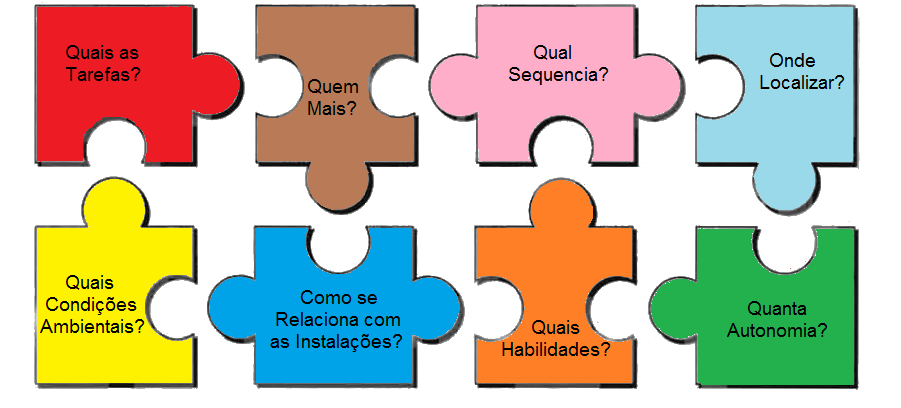
\includegraphics[scale=0.6]{organizacao1}
			\caption[Elementos do projeto do trabalho]{Elementos do Projeto do Trabalho. \cite{slack}}
			\label{fig:organizacao1}
		\end{figure}

		As diferentes respostas para cada elemento do projeto do trabalho descritas têm implicações sobre as habilidades e capacidades que as pessoas irão necessitar para desempenhar seus trabalhos efetivamente e é daqui que surge a sua importância de ser bem consolidada numa empresa. Cabe ressaltar que os objetivos de desempenho ainda possuem relevância nas decisões de projeto de trabalho, são eles:

		\begin{itemize}
			\item{\textbf{Qualidade}: a habilidade do pessoal em produzir produtos e serviços de alta qualidade pode ser afetada pelo projeto de trabalho;}
			\item{\textbf{Rapidez}: algumas vezes, a velocidade de resposta é o: objetivo predominante no projeto de trabalho;}
			\item{\textbf{Confiabilidade}: o projeto de trabalho deve enfatizar a confiança do fornecimento do produto/serviço;}
			\item{\textbf{Flexibilidade}: o projeto de trabalho deve permitir a flexibilidade na execução das atividades;}
			\item{\textbf{Custo}: projeto de trabalho influencia a produtividade e o custo.}
		\end{itemize}

		Agora, tendo em vista as abordagens práticas do projeto de trabalho, pode dizer que há várias abordagens, no qual, ao longo dos anos diferenciaram-se entre e tem influências em diferentes momentos. Nenhuma delas é mutuamente exclusiva, mas representam diferentes filosofias ou, pelo menos, enfatizam diferentes aspectos do projeto do trabalho. A imagem a seguir ilustra de forma cronologia a essas abordagens.

		\begin{figure}[h]
			\centering
			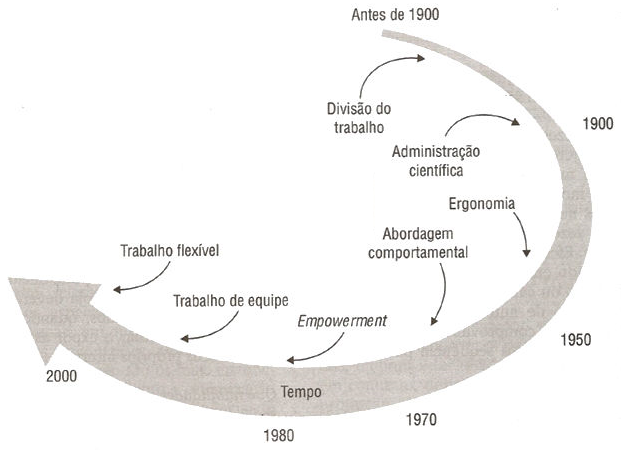
\includegraphics[scale=0.8]{organizacao2}
			\caption[Cronologia das diferentes abordagens para o Projeto de Trabalho]{Cronologia das diferentes abordagens para o Projeto de Trabalho. \cite{slack}}
			\label{fig:organizacao2}
		\end{figure}

	\section[Aplicações]{Aplicações - 
\includegraphics{bobs2}}
	\label{sec:organizacao_aplicacoes}

		A rede \textbf{Bob’s} possui um departamento de recursos humanos segundo a entrevista com o gerente da equipe. Isso porque, todos os funcionários são bem treinados a capacitados para desempenhar suas atividades. Além disso, o \textbf{Bob’s} oferece a possibilidade de plano de carreira, como é o caso do gerente de equipe que começou utilizando aquele boné e fritando muitos hambúrgueres, mas depois de alguns anos de dedicação teve sua tão sonhada promoção. 
		
		A empresa, ao contratar novas funcionários, oferecem o treinamento técnico para compreensão das habilidades e capacidades necessárias para o exercício da função e o treinamento prática coordenado por um gerente, no qual o recém contratado pratica as questões discutidas no treinamento técnico. O início não costuma ser imediato, pois é necessário que o funcionário obtenha uma experiência mínima, isso devido a demanda de cliente, no qual exige uma certa rapidez durante a produção. Essa é uma regra de negócio estabelecida pela empresa, pois, assume-se o lado tanto do novo funcionário com o medo inerente a inexperiência, quanto ao cliente que não necessitará esperar um tempo maior a produção de um produto pelo novo funcionário.

		\subsection[Divisão de Trabalho]{Divisão de Trabalho}
		\label{sec:organizacao_dt}

			A empresa em si já trabalha com a produção de produtos em diferentes disposições no local físico, como observado no capitulo \ref{chap:arranjo} (\nameref{chap:arranjo}). Existe a produção de \emph{milk shakes}, que é diferente da produção de Sanduiches, que é diferente da produção de pratos prontos e assim por diante. Essa distribuição dá autonomia para que os funcionários possam trabalhar sem estarem preocupados uns com os outros, mas sim, com a sua função para produção do produto. Agora, a desvantagem desse sistema adotado é o grau de repetitividade da operação, ou seja, o trabalho acaba ficando monótono. Mas, para resolver este problema, a \textbf{Bob’s} adota a abordagem em equipe, no qual será discutida posteriormente.

		\subsection[Administração Científica]{Administração Científica}
		\label{sec:organizacao_ac}

			A rede \textbf{Bob’s} possui em sua matriz, tanto de São Paulo quanto do Rio de Janeiro, equipe de administração cientifica, que são responsáveis pelos estudos das tendências mundiais para os \emph{fast foods}, marketing inteligente, questões ergonômicas no trabalho, saúde coletiva entre algumas outras. Essas questões são importantes, pois de acordo com os estudos, modificações vão sendo, aos poucos, implantadas nas redes com o objetivo de atendendo melhor o cliente, e proporcionar um ambiente no mínimo agradável aos funcionários. \cite{osman}

		\subsection[Ergonomia]{Ergonomia}
		\label{sec:organizacao_ergonomia}

			Para cada espaço físico a ser construído um arranjo físico do \textbf{Bob’s} existe um modelo ergonômico adaptado para o mesmo. Como ilustrado no arranjo físico do \textbf{Bob’s} no \textbf{Taguatinga Shopping}, as passagens para o fluxo de pessoas foram pensadas para que os funcionários passassem com o maior conforto possível de acordo com o espaço disponível. Uma questão levantada durante a entrevista com o gerente foi o calor produzido pelo preparo dos produtos, pois como o espaço era relativamente pequeno com uma quantidade grande de pessoas, as condições humanas possivelmente seriam insuportáveis. No entanto, para resolver este problema a empresa disponha de tecnologia de resfriamento do ambiente, para isso eram utilizados ar condicionados e outra tecnologia de captura do ar quente, que fica na parte superior do teto da cozinha.

			Apesar das questões levantadas anteriormente serem validas, ainda foi possível percebe que a maioria dos funcionários trabalham em pé, exceção apenas para o caixa de atendimento de solicitações de pedido. Essa observação foi questionada pelo gerente justificando que, por causa das condições físicas, principalmente o espaço físico, isso não era possível, possui as cadeiras poderiam tornar os espaços para fluxo de pessoas muito menor do que já era, prejudicando o bom andamento do processo. Além do mais, os funcionários de produção dos produtos, não estão estáticos durante a produção, pois na maioria das vezes, eles precisam de pequenos deslocamentos na “\emph{esteira de produção}” para pegar algum produto ou material.

		\subsection[Abordagens Comportamentais e Empowerment]{Abordagens Comportamentais e \emph{Empowerment}}
		\label{sec:organizacao_ace}

			A empresa possui políticas de valorização dos funcionários, inclusive plano de carreiras para os funcionários que possui destaque sem seu trabalho. O exemplo prático disso é a utilização do quadro de funcionário do mês, no qual, são elegidos os melhores funcionários do mês obedecendo uma série de critérios como produtividade, responsabilidade, faltas entre outros critérios. Com essa metodologia, o gerente de equipe acredita que é mais fácil promover a responsabilidade individual dos funcionários com relação ao trabalho, fazendo com que o desempenho geral da rede caminhe bem. Além disso, as equipes de trabalho, uma vez por semestre saem para desfrutar de um ambiente não corporativo, isso segundo o gerente, faz com que os funcionários deixem de lado o estresse as vezes acumulados durante o trabalho. \cite{junior}

		\subsection[Trabalho em Equipe e Trabalho Flexível]{Trabalho em Equipe e Trabalho Flexível}
		\label{sec:tecnologias_tetf}

			Esses são dos dois pontos chaves para redes \textbf{Bob’s} segundo o gerente de equipe. Todo o sistema da rede funciona com equipes funcionais com alguns papeis rotativos de acordo com as escalas montadas. Para o gerente, quando o funcionário de produção de hambúrgueres troca seu papel com o funcionário de produção de pratos prontos, as experiências em ambas as funções são distribuídas por toda a equipe, além do mais o stress produzido por ambas as funções é minimizado por essa rotatividade. Essa característica aumenta a produtividade e a satisfação por parte dos funcionários, aumenta a qualidade dos produtos produzidos e proporciona flexibilidade, pois as equipes trabalham por escalas que são organizadas de acordo com as necessidades por meio de uma reunião com os gerentes de equipes. 
